\documentclass{article}
\usepackage{graphicx}
\usepackage[english,greek]{babel}
\usepackage[utf8x]{inputenc}
\usepackage{amsmath}
\usepackage{relsize}
\usepackage{enumerate}
\usepackage[parfill]{parskip}
\usepackage{graphicx}

\makeatletter
\renewcommand*\env@matrix[1][*\c@MaxMatrixCols c]{%
  \hskip -\arraycolsep
  \let\@ifnextchar\new@ifnextchar
  \array{#1}}
\makeatother

\begin{document}

\title{\vspace{-3.5cm}\textbf{Προστασία και Ασφάλεια Υπολογιστικών Συστημάτων \\ΕΑΡΙΝΟ 2018\\ \textlatin{Project \#}1}}
\author{Λάμπρου Ιωάννης \\1115201400088\\\\ Στεφανίδης - Βοζίκης Κωνσταντίνος \\1115201400192}

\maketitle
\section*{\textlatin{Defence}}
\subsection*{\textlatin{CSRF}}
Όσον αφορά την άμυνα για τις επιθέσεις \textlatin{CSRF}. Ποστατευθήκαμε βάζοντας \textlatin{CSRF tokens} 
σε κάθε φόρμα ή οποία προκαλεί αλλαγές στην σελίδα. Σε κώδικα \textlatin{PHP} ή άμυνα μοιάζει κάπως 
έτσι:\\
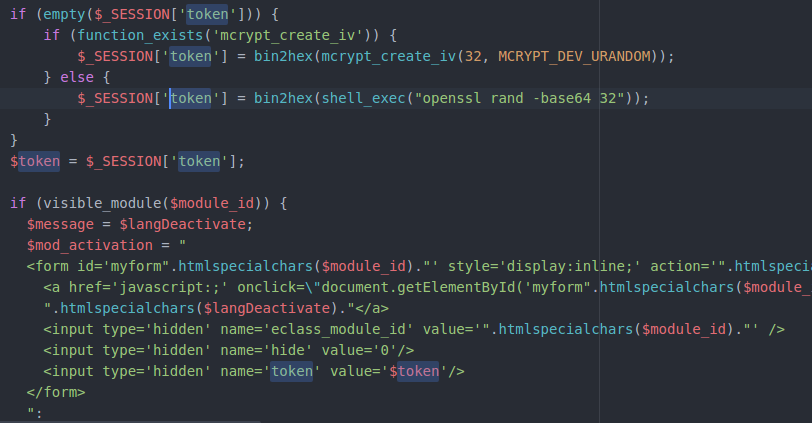
\includegraphics[scale=0.5]{csrf}\\
Πρώτα ενεργοποιούμε ενα \textlatin{token} και κατόπιν το βάζουμε ως \textlatin{hidden field} στην 
φόρμα που μας ενδιαφέρει. Ο έλεγχος εγκυρότητας γίνεται ως εξης:\\
\textlatin{if (isset(\$\_POST['hide']) and \$\_POST['hide'] == 0 and !empty(\$\_POST['token']) and (strcmp(\$\_SESSION['token'], \$\_POST['token']) === 0))}\\
Η ίδια λογική άμυνας υπάρχει σε κάθε φόρμα της ιστοσελίδας (η οποία προκαλεί αλλαγές).
Επίσης, επειδή δεν υπάρχει άμυνα έναντι επιθέσεων \textlatin{CSRF} σε \textlatin{GET requests}, διάφορα 
\textlatin{GET} που άλλαζαν την σελίδα αλλάχθηκαν σε \textlatin{POST} ώστε να γίνει η ίδια άμυνα. 
Ένα παράδειγμα είναι η διαγραφή χρήστη από την σελίδα του \textlatin{admin}.
%\begin{enumerate}
%\item



\section*{\textlatin{Attack}}
\begin{enumerate}[(a)]%for small alpha-characters within brackets.
\item
Σωστό. Το $\omega{()}$ είναι αυστηρότερο, άρα και η $f(x)$ θα είναι και  Ω$(g(n))$ (Αφού το Ω είναι υπερσύνολο του ω)
\item
Λάθος. Για $n > 1$, πάντα η$(10n^2 + kn + c)$ θα είναι μεγαλύτερη ή ίση από τη $(4n^2 + 5n - 9)$ $(4n^2 + 5n - 9) = O(10n^2)$ 
\item
Σωστό. Ξέρουμε από τις διαφάνειες πως $\log{n!} = O(n\log{n})$ (Άσκηση 4, σελ 15), ενώ $\log{n!} = \log{1} + \log{2} + ... + \log{n} >= \\\\
 \log{\frac{n}{2}} + \log{\frac{n}{2}+1} + ... + \log{n} = \log{\frac{n}{2}}*\frac{n}{2} = \frac{n\log{n}}{2}-\frac{n\log{2}}{2} =>\\\\
\log{n!} >=  \frac{n\log{n}}{2}-\frac{n\log{2}}{2}$, Άρα και $\log{n!}$ $=$Ω$(n\log{n})$. Αφού  το $\log{n!}$ είναι και Ο και Ω του $(n\log{n})$, τότε θα είναι και Θ
\item
Λάθος. Ξέρουμε πως $f(n) + g(n) = $Ω$(min(g(n),f(n)))$ ενώ $f(n) + g(n) = O(max(g(n),f(n)))$ άρα ισχύει μόνο στην περίπτωση που $f(n) = g(n)$
\item
Σωστό. Αν πάρουμε το όριο, $ lim_{n\to\infty} \frac{n+2\sqrt{n}}{n\sqrt{n}} = lim_{n\to\infty} \frac{\sqrt{n}+2}{n} = 0$, άρα είναι O
\item
Σωστό. Ξέρουμε ότι το όριο $ lim_{n\to\infty} (g(n) - f(n)) = -\infty$. Αν πάρουμε το όριο, $ lim_{n\to\infty} \frac{2^{g(n)}}{2^{f(n)}} =  lim_{n\to\infty} 2^{g(n)-f(n)}$ το οποίο και θα κάνει μηδέν, λόγω του αρχικού ορίου. Άρα και το $2^{f(n)}$ θα είναι Ω$(2^{g(n)})$ άρα και ω.
\item
Σωστό. Αποδείχτηκε στο προηγούμενο ερώτημα.
\item
Σωστό. Έστω $f(x) = $ω$(g(x)$, τότε θα πρέπει για $x>=x_0 f(x) > g(x)$. Ομοίως, αν $f(x) = $ο$(g(x)$, τότε θα πρέπει για $x>=x_0 f(x) < g(x)$ Έτσι, βλέπουμε ότι τα δύο αυτά ενδεχόμενα είναι ξένα.

\end{enumerate}
\end{document}